%-----------------------------------------------------------------------------
%
%               Template for sigplanconf LaTeX Class
%
% Name:         sigplanconf-template.tex
%
% Purpose:      A template for sigplanconf.cls, which is a LaTeX 2e class
%               file for SIGPLAN conference proceedings.
%
% Guide:        Refer to "Author's Guide to the ACM SIGPLAN Class,"
%               sigplanconf-guide.pdf
%
% Author:       Paul C. Anagnostopoulos
%               Windfall Software
%               978 371-2316
%               paul@windfall.com
%
% Created:      15 February 2005
%
%-----------------------------------------------------------------------------


\documentclass[preprint,numbers]{sigplanconf}

% The following \documentclass options may be useful:

% preprint      Remove this option only once the paper is in final form.
% 10pt          To set in 10-point type instead of 9-point.
% 11pt          To set in 11-point type instead of 9-point.
% numbers       To obtain numeric citation style instead of author/year.

\usepackage{amssymb}
\usepackage{amsmath}
\usepackage{amsfonts}
\usepackage{caption}
\usepackage{subcaption}
\usepackage{xspace}
\usepackage{mathtools}
\usepackage{mathpartir}
\usepackage{ifpdf}
\usepackage{graphicx}
\usepackage[usenames,dvipsnames]{color}
\usepackage{stmaryrd}
%\usepackage[numbers]{natbib}
\usepackage{amsthm}
\usepackage{listings}          % format code
\usepackage{wrapfig}
\usepackage{textcomp}
\usepackage{tabularx}
\usepackage{color}


% Math mode
%-----------
\newenvironment{nop}{}{}
\newenvironment{smathpar}{
\begin{nop}\small\begin{mathpar}}{
\end{mathpar}\end{nop}\ignorespacesafterend}

% Theorem
%--------

% \theoremstyle{plain}
% \newtheorem{axiom}{Axiom}[section]
% \newtheorem{theorem}{Theorem}[section]
% \newtheorem{lemma}[theorem]{Lemma}
% \newtheorem{proposition}[theorem]{Proposition}
% \newtheorem{corollary}[theorem]{Corollary}
% \theoremstyle{definition}
% \newtheorem{definition}[theorem]{Definition}

% \newenvironment{example}[1][Example]{\begin{trivlist}
% \item[\hskip \labelsep {\bfseries #1}]}{\end{trivlist}}
% \newenvironment{remark}[1][Remark]{\begin{trivlist}
% \item[\hskip \labelsep {\bfseries #1}]}{\end{trivlist}}

% Decorations
%-----------
\newenvironment{decoration}
  {\color{blue}\begin{array}{l}}
  {\end{array}}

% New colors
%------------
\definecolor{Bittersweet}{rgb}{1.0, 0.44, 0.37}
\definecolor{MidnightBlue}{rgb}{0.0, 0.2, 0.4}

% Listings
%----------
\newcommand{\lsttxnimp}{\lstset{
      language=c,
      basicstyle=\ttfamily\small,
      flexiblecolumns=false,
			tabsize=2,
      escapechar=',                        
      %basewidth={0.5em,0.45em},
      %aboveskip={3pt},
      %belowskip={3pt},
      keywordstyle=\color{Bittersweet}\bfseries,
      commentstyle=\color{blue}\itshape,
      stringstyle=\color{MidnightBlue},
      morekeywords={transaction,txn,cobegin,from,to,atomic},
			classoffset=1,
			upquote=true,
			keywordstyle=\color{Fuchsia}\bfseries,
			classoffset=0,
			mathescape=true
    }}
\lstnewenvironment{txnimpcode}
    { % \centering
      \lsttxnimp
      \lstset{}%
      \csname lst@setfirstlabel\endcsname}
    { %\centering
      \csname lst@savefirstlabel\endcsname}

% Listings Code
%---------------
\newcommand{\lstml}{
\lstset{ %
language=ML, % choose the language of the code
basicstyle=\footnotesize\ttfamily,       % the size of the fonts that are used for the code
keywordstyle=\color{Bittersweet},
% numbers=left,                   % where to put the line-numbers
numberstyle=\tiny,      % the size of the fonts that are used for the line-numbers
stepnumber=1,                   % the step between two line-numbers. If it is 1 each line will be numbered
numbersep=5pt,                  % how far the line-numbers are from the code
showspaces=false,               % show spaces adding particular underscores
showstringspaces=false,         % underline spaces within strings
showtabs=false,                 % show tabs within strings adding particular underscores
% frame=single,                   % adds a frame around the code
tabsize=2,                      % sets default tabsize to 2 spaces
captionpos=b,                   % sets the caption-position to bottom
breaklines=true,                % sets automatic line breaking
breakatwhitespace=false,        % sets if automatic breaks should only happen at whitespace
commentstyle=\itshape\color{MidnightBlue},
%escapeinside={\%*}{*)},         % if you want to add a comment within your code
mathescape=true,
morekeywords={module, match, when, @@deriving, not, : , txn_do, do, SQL/\\}
}}
\lstnewenvironment{ocaml}
    { % \centering
			\lstml
      \lstset{}%
      \csname lst@setfirstlabel\endcsname}
    { %\centering
      \csname lst@savefirstlabel\endcsname}
\newcommand{\ocamlinline}[1]{\lstinline[language=ML,
                                        basicstyle=\footnotesize\ttfamily, 
                                        keywordstyle=\color{Bittersweet},
                                        mathescape=true]{#1}}

% Formatting
%---------
\newcommand{\C}[1]{\code{#1}}
%\newcommand{\R}[1]{\textsc{#1}}
\newcommand{\tuplee}[1]{\langle #1 \rangle}
\newcommand*{\rom}[1]{\expandafter\romannumeral #1}

% Formatting commands
% -------------------
\newcommand{\code}[1]{{\tt #1}}
\newcommand{\spc}[0]{\quad}
\newcommand{\ALT}{~\mid~}
\newcommand{\rel}[1]{{R}_{\mathit{#1}}}
\newcommand{\conj}{~\wedge~}
\newcommand{\disj}{~\vee~}
\newcommand{\rulelabel}[1]{\textrm{\sc {#1}}}
\newcommand{\ilrulelabel}[1]{{\sc #1}}
\newcommand{\RULE}[2]{\frac{\begin{array}{c}#1\end{array}}
                           {\begin{array}{c}#2\end{array}}}
\newcommand{\txnimp}{\mbox{${\mathcal T}$}}
%\newcommand{\coloneqq}{::=}
\newcommand{\qqquad}{\quad\quad}
\newcommand{\cskip}{\C{SKIP}}
\newcommand{\ctxnr}[3]{{\sf txn}_{#1}\langle #2 \rangle\{#3\}}
\newcommand{\ctxn}[3]{\C{TXN}_{#1}\langle #2 \rangle\{#3\}}
\newcommand{\catomic}[1]{\C{ATOMIC}\{#1\}}
\newcommand{\stepsto}{\longrightarrow}
\newcommand{\rstepsto}{\longrightarrow_{R}}
\newcommand{\stepssto}[1]{\longrightarrow^{#1}_{R}}
\newcommand{\rstepssto}[1]{\longrightarrow^{#1}_{R}}
\newcommand{\xstepsto}[1]{\longrightarrow_{#1}}
\newcommand{\xstepssto}[2]{\longrightarrow^{#1}_{#2}}
\newcommand{\tstepsto}{\longrightarrow}
\newcommand{\redsto}{\hookrightarrow}
\newcommand{\xtstepsto}[1]{\hookrightarrow_{#1}}
\newcommand{\rtstepsto}{\hookrightarrow_R}
\newcommand{\rtstepssto}[1]{\hookrightarrow^{#1}_R}
\newcommand{\xtstepssto}[2]{\hookrightarrow^{#1}_{#2}}
\newcommand{\hoare}[3]{\{#1\}\,#2\,\{#3\}}
\newcommand{\defeq}[0]{\overset { \mathit{def} }{ = } }
\newcommand{\rg}[3]{\{#1\}\,#2\,\{#3\}}
%\newcommand{\defeq}[0]{ \triangleq }
\newcommand{\op}{\textsf{op}}
\newcommand{\E}{\textsf{E}}
\newcommand{\A}{\textsf{A}}
\newcommand{\I}{\mathbb{I}}
\newcommand{\R}{\mathbb{R}}
\newcommand{\F}{{\sf F}}
\newcommand{\visZ}{\textsf{vis}}
\newcommand{\soZ}{\textsf{so}}
\newcommand{\hbZ}{\textsf{hb}}
\newcommand{\sameobj}[2]{\textsf{sameobj}(#1,#2)}
\newcommand{\sameobjZ}{\textsf{sameobj}}
\newcommand{\visar}{\xrightarrow{\visZ}}
\newcommand{\hboar}{\xrightarrow{\textsf{hb}}}
\newcommand{\soar}{\xrightarrow{\soZ}}
\newcommand{\visoar}{\xrightarrow{\visZ \,\cup\, \soZ}}
\newcommand{\invisar}{\xrightarrow{\textsf{invis}}}
\newcommand{\etaar}{\xrightarrow{\eta}}
\newcommand{\wrstoar}{\xrightarrow{\textsf{wrsto}}}
\newcommand{\rdsfmar}{\xrightarrow{\textsf{rdsfm}}}
\newcommand{\usesar}{\xrightarrow{\textsf{uses}}}
\newcommand{\isReadf}{\textsf{isRD}}
\newcommand{\isWritef}{\textsf{isWR}}
\newcommand{\oper}{\textsf{oper}}
\newcommand{\committed}{\textsf{com}}
\newcommand{\txn}{\textsf{txn}}
\newcommand{\id}{\textsf{id}}
\newcommand{\kind}{\textsf{oper}}
\newcommand{\rval}{\textsf{rval}}
\newcommand{\visible}{\textsf{visible}}
\newcommand{\maxId}{\textsf{maxId}}
\newcommand{\eval}{\textsf{eval}}
\newcommand{\dom}{\textsf{dom}}
\newcommand{\uid}{\textsf{id}}
\newcommand{\underE}[1]{\E \Vdash #1}
\newcommand{\underIT}[1]{\;\I,\C{Txn}_i \vdash #1\;}
\newcommand{\underI}[1]{\;\I \vdash #1\;}
\newcommand{\underT}[1]{\;\C{Txn}_i \vdash #1\;}
\newcommand{\stable}{\mathtt{stable}}
\newcommand{\iso}[1]{\emph{#1}}
\newcommand{\writef}{\textsf{Write}}
\newcommand{\readf}{\textsf{Read}}
\newcommand{\commitf}{\textsf{Commit}}
\newcommand{\eg}{\emph{e.g.,}}
\newcommand{\GK}[1]{\textcolor{red}{GK: #1}}
\newcommand{\SJ}[1]{\textcolor{red}{SJ: #1}}

\newcommand{\B}[1]{\small\bf #1}
\newcommand{\tbox}[1]{\lbrack #1 \rbrack}
\newcommand{\interp}[1]{\llbracket #1 \rrbracket}
\newcommand{\cinterp}[1]{\llbracket #1 \rrbracket_{\C{C}}}
\newcommand{\ectx}{\mathcal{E}}
\newcommand{\isMax}{\textsf{isMax}}
\newcommand{\Prop}{\mathbb{P}}
\newcommand{\Pow}[1]{\mathcal{P}\left(#1\right)}
\newcommand{\bind}{\gg=}
\newcommand{\ite}[3]{\C{IF}\;#1\;\C{THEN}\;#2\;\C{ELSE}\;#3}
\newcommand{\lete}[3]{\C{LET}\;#1=#2\;\C{IN}\;#3}
\newcommand{\foreache}[2]{\texttt{FOREACH}\;#1\;\texttt{DO}\;#2}
\newcommand{\foreachr}[3]{{\sf foreach}\langle #1 \rangle\;#2\;{\sf do}\;#3}
\newcommand{\inserte}[1]{\texttt{INSERT}\;#1}
\newcommand{\selecte}[1]{\texttt{SELECT}\;#1}
\newcommand{\deletee}[1]{\texttt{DELETE}\;#1}
\newcommand{\updatee}[2]{\texttt{UPDATE}\;#1\;#2}
\newcommand{\stl}{\delta}
\newcommand{\stg}{\Delta}
\newcommand{\rec}{r}
\newcommand{\idf}{\texttt{id}}
\newcommand{\delf}{\texttt{del}}
\newcommand{\txnf}{\texttt{txn}}
\newcommand{\eff}{\mathcal{F}}
\newcommand{\elabsto}{\Longrightarrow_{\langle i,\R,I \rangle}}
\newcommand{\with}{~\C{with}~}
\newcommand{\itel}[3]{{\sf if}\;#1\;{\sf then}\;#2\;{\sf else}\;#3}
\newcommand{\stabilize}[1]{\llfloor #1 \rrfloor_{\langle \R,I \rangle}}
\newcommand{\semof}[1]{\llbracket #1 \rrbracket}
\newcommand{\mssemof}[1]{\llbracket #1 \rrbracket_{\Vdash}}
\newcommand{\existsl}{{\sf exists}}
\newcommand{\fresh}{{\sf fresh}}
\newcommand{\SL}{\mathcal{S}}


\begin{document}

\special{papersize=8.5in,11in}
\setlength{\pdfpageheight}{\paperheight}
\setlength{\pdfpagewidth}{\paperwidth}

\conferenceinfo{CONF 'yy}{Month d--d, 20yy, City, ST, Country}
\copyrightyear{20yy}
\copyrightdata{978-1-nnnn-nnnn-n/yy/mm}
\copyrightdoi{nnnnnnn.nnnnnnn}

% Uncomment the publication rights you want to use.
%\publicationrights{transferred}
%\publicationrights{licensed}     % this is the default
%\publicationrights{author-pays}


\title{Working Title: Compositional Reasoning for Weakly Isolated Transactions }

\authorinfo{} {} {}
\maketitle

\begin{abstract}

  Serializability is a well-understood correctness criterion that
  simplifies reasoning about the behaviour of concurrent transactions
  by ensuring they are \emph{isolated} from each other while they
  execute.  However, enforcing serializable isolation comes at a steep
  cost in performance because it necessarily restricts opportunities
  to exploit concurrency even when such opportunities would not
  violate application-specific invariants. As a result, database
  systems in practice support, and often encourage, developers to use
  weaker alternatives. These alternatives break the strong isolation
  guarantees offered by serializable transactions to permit greater
  concurrency. Unfortunately, the semantics of weak isolation is
  poorly understood, and usually explained only informally in terms of
  low-level implementation artifacts. Consequently, verifying
  high-level correctness properties in such environments remains a
  challenging problem.

  To address this issue, we present a program logic that enables
  compositional reasoning about the behaviour of concurrently
  executing weakly-isolated transactions. Notably, our development is
  parametric over a transaction's specific isolation semantics, and
  the consistency guarantees provided by the underlying data store,
  allowing it to be applicable over a range of concurrency control
  mechanisms.  Case studies and experiments on real-world applications
  demonstrate the utility of our approach, and provide strong evidence
  that weakly-isolated transactions can be placed on the same formal
  footing as their strongly-isolated serializable counterparts.

\end{abstract}



\section{Introduction}

Database transactions allow users to group operations on multiple
objects into a single logical unit, equipped with a set of four key
properties - atomicity, consistency, isolation, and durability (ACID).
Concurrency control mechanisms provide specific instantiations of
these properties to yield different ACID variants that characterize
how and when the effects of concurrently executing transactions become
visible to one another.  \emph{Serializability} is a particularly
well-studied instantiation that imposes strong atomicity and isolation
constraints on transaction execution, ensuring that any permissible
concurrent schedule yields results equivalent to a serial one in which
there is no interleaving of actions from different transactions.

The guarantees provided by serializability do not come for free,
however - pessimistic concurrency control methods require databases to
use expensive mechanisms such as two-phase locking that incur overhead
to deal with deadlocks, rollbacks, and
re-execution~\cite{twopl,ullmanbook}.  Similar criticisms apply to
optimistic multi-version concurrency control methods that must deal
with timestamp and version management~\cite{BG81}.  These issues are
further exacerbated when the database is replicated, requiring
additional coordination
mechanisms~\cite{cap,sernotavlbl,bailishat,bernsigmod13}.

Because serializable transactions favor correctness over performance,
there has been long-standing interest~\cite{gray1976} in the database
community to consider weaker variants that try to recover performance,
even at the expense of simplicity and ease of reasoning.  These
instantiations permit a transaction to witness various effects of
newly committed, or even concurrently running, transactions while it
executes, thus weakening serializability's strong isolation
guarantees.  The ANSI SQL 92 standard defines three such weak
isolation levels which are now implemented in many relational and
NoSQL databases. Not surprisingly, weakly-isolated transactions have
been found to significantly outperform serializable transactions on
benchmark suites, both on single-node databases and multi-node
replicated stores~\cite{dbtuningbook,bailishat,bailisvldb}, leading to
their overwhelming adoption. A 2013 study~\cite{bailishotos} of 18
popular ACID and ``NewSQL'' databases found that only three of them
offer serializability by default, and half, including Oracle 11g, do
not offer it at all.  A 2015 study~\cite{bailisferal} of a large
corpus of database applications finds no evidence that applications
manifestly change the default isolation level offered by the
database. Taken together, these studies make clear that
weakly-isolated transactions are quite prevalent in practice, and
serializable transactions are often eschewed.

Unfortunately, weak isolation admits behaviors that are difficult to
comprehend~\cite{berenson}. To quantify weak isolation anomalies,
Fekete \emph{et al.}~\cite{feketevldb09} devised and experimented with
a microbenchmark suite that executes transactions under a
weakly-isolated \emph{read committed} isolation level - the default
level for 8 of the 18 databases studied in~\cite{bailishotos}, and
found that 25 out of every 1000 rows in the database violate at least
one integrity constraint. Bailis \emph{et al.}~\cite{bailisferal} rely
on Rails' \emph{uniqueness validation} to maintain uniqueness of
records while serving Linkbench's~\cite{linkbench} insertion workload
(6400 records distributed over 1000 keys; 64 concurrent clients), and
report discovering more than 10 duplicate records.  Rails relies on
database transactions to validate uniqueness during insertions, which
is sensible if transactions are serializable, but incorrect under the
weak isolation level used in the experiments. The same study has found
that 13\% of all invariants among 67 open source Ruby-on-Rails
applications are at risk of being violated due to weak
isolation. Indeed, incidents of safety violations due to executing
applications in a weakly-isolated environment have been reported on
web services in production~\cite{starbucksbug, scimedbug}, including
in safety-critical applications such as bitcoin
exchanges~\cite{poloniexbug, bitcoinbug}. While enforcing
serializability for all transactions would be sufficient to avoid
these errors and anomalies, it would likely be an overly conservative
strategy; indeed, 75\% of the invariants studied in~\cite{bailisferal}
were shown to be preserved under some form of weak isolation.  When to
use weak isolation, and in what form, is therefore a prominent
question facing all database programmers.\footnote{This position has
been echoed by database researchers who lament the lack of a
better understanding of this problem; see e.g., {\tt
  http://www.bailis.org/blog/understanding-weak-isolation-is-a-serious-problem}.}

A major problem with weak isolation as currently specified is that its
semantics in the context of user programs is not easily
understood. The original proposal~\cite{gray1976} defines multiple
``degrees'' of weak isolation in terms of implementation details such
as the nature and duration of locks held in each case. The ANSI SQL 92
standard defines four levels of isolation (including serializability)
in terms of various undesirable \emph{phenomena} (\eg \emph{dirty
  reads} - reading data written by an uncommitted transaction) each is
required to prevent. While this is an improvement, this style of
definition still requires programmers to be prescient about the
possible ways various undesirable phenomena might manifest in their
applications, and in each case determine if the phenomenon can be
allowed without violating application invariants. This is
understandably hard, especially in the absence of any formal
underpinning to define weak isolation semantics.  Adya~\cite{adyaphd}
presents the first formal definitions of some well-known isolation
levels in the context of a sequentially consistent (SC) database.
However, there has been little progress relating Adya's system model
to a formal operational semantics or a proof system that can
facilitate rigorous correctness arguments.  Consequently, reasoning
about weak isolation remains an error prone endeavor, with major
database vendors~\cite{postgresiso, mysqliso, oracleiso} continuing to
document their isolation levels primarily in terms of the undesirable
phenomena a particular isolation level may induce, placing the burden
on the programmer to determine application correctness.

Recent results on reasoning about application invariants in the
presence of weak consistency~\cite{burckhardt14, redblueosdi,
  redblueatc, ecinec, gotsmanpopl16} address broadly related concerns.
Weak consistency is a phenomenon that manifests on replicated data
stores, where atomic operations are concurrently executed against
different replicas, resulting in an execution order inconsistent with
any sequential order. In contrast, weak isolation is a property of
concurrent transactions interfering with one another, resulting in an
execution order that is not serializable. Unlike weak consistency,
weak isolation can manifest even in an unreplicated setting, as
evident from the support for weakly-isolated transactions on
conventional (unreplicated) databases as mentioned above.

%% In the
%% presence of replication, however, the interaction between weak
%% isolation and weak consistency can be subtle and non-trivial.
%% Understanding weak isolation in these varied contexts thus requires
%% new insights and substantial generalization of existing techniques.

%% Recent results on reasoning about application invariants in the
%% presence of weak consistency~\cite{burckhardt14, redblueosdi,
%% redblueatc, ecinec, gotsmanpopl16} address broadly related concerns.
%% Weak consistency is a phenomenon that usually manifests on replicated
%% data stores, where operations are concurrently executed against
%% different replicas, resulting in an order of execution inconsistent
%% with their serial order. The operations, nonetheless, are atomic and
%% fully isolated, and each operation is required to locally preserve
%% application invariants. In contrast, weak isolation is a property of
%% transactions, which are sets of atomic operations. Weak isolation
%% manifests when successive atomic operations in a transaction witness
%% different contemporary states of the database (or different replicas
%% of the replicated store) which, although consistent individually, may
%% not be obviously reconciled into a consistent global view.
%% Intuitively, the latter problem reduces to the former if all
%% transactions contain a single operation. Furthermore, weak isolation
%% can exist independent of weak consistency, as evident from the
%% presence of weakly-isolated transactions on conventional RDBS. With an
%% added complexity of replication, richer mechanisms are needed to
%% reason about weak isolation in tandem with weak consistency. Thus,
%% frameworks for reasoning about weak isolation will necessarily have to
%% generalize the reasoning frameworks developed for weak consistency in
%% new and important ways.

% The framework should be general enough to reason about the semantics
% of multiple isolation levels, including those proposed after the SQL
% 92 standard, in the context of various stores (\eg sequentially
% consistent store of~\cite{adyaphd}, causally consistent store
% of~\cite{gotsmanpopl16} etc). 

In this paper, we propose a program logic for weakly-isolated
transactions along with automated verification support to allow
developers to verify the soundness of their applications, without
having to resort to low-level operational reasoning as they are forced
to do currently.  We develop a set of syntax-directed compositional
proof rules that enable the construction of correctness proofs for
transactional programs in the presence of a weakly-isolated
concurrency control mechanism.  Realizing that the proof burden
imposed by these rules may discourage applications programmers from
using them, we also present an inference procedure based on these
rules that automatically verifies the weakest isolation level for a
transaction that still ensures its invariants are maintained.  The key
to inference is a novel formulation of database state (represented as
sets of tuples) as a monad, and in which database computations are
interpreted as state transformers over these sets.  This
interpretation leads to an encoding of database computations amenable
for verification by off-the-shelf SMT solvers.  The paper makes the
following contributions:
%% We have realized these ideas as an embedded DSL within OCaml, that
%% supports common relational SQL operations (updates, selects, inserts,
%% deletes, joins, etc.).  Experimental results on real-world benchmarks
%% demonstrate the feasibility and value of automated verification for
%% weakly isolated transactions, an important advance in improving the
%% safety of realistic database computations.
\begin{enumerate}
  \item We analyze properties of weak isolation in the context of a
    DSL embedded in OCaml that treats SQL-based relational database
    operations (e.g., inserts, selects, deletes, updates, etc.) as
    computations over an abstract database state.
  \item We develop an operational semantics and a compositional
    rely-guarantee style proof system for this language capable of
    relating high-level application invariants to database state,
    parameterized by a weak isolation semantics that selectively
    exposes the visibility of these operations to other transactions.
  \item We devise an inference algorithm capable of discovering the
    weakest isolation level that is sound with respect to a
    transaction's high-level consistency requirements. The algorithm
    interprets database operations as state transformers expressed in
    a language amenable for translation into a decidable fragment of
    first-order logic, and is thus suitable for automated verification
    using off-the-shelf SMT solvers.
  \item We present details of an implementation along with an
    evaluation study on real database benchmarks that justify our
    approach, and demonstrate the utility of our inference mechanism.
\end{enumerate}
\noindent Our results provide the first (to the best of our knowledge)
formalization of weakly-isolated transactions, along with an
expressive and compositional proof automation framework capable of
verifying the safety of high-level consistency conditions attached to
these transactions.  Collectively, these contributions allow
weakly-isolated transactions to enjoy the same rigorous reasoning
capabilities as their strongly-isolated (serializable) counterparts.

The remainder of the paper is organized as follows. The next section
provides motivation and background on serializable and weakly-isolated
transactions. \S\ref{sec:opsem} presents an operational semantics for
a core language that supports weakly-isolated transactions,
parameterized over different isolation notions. \S\ref{sec:reasoning}
formalizes the proof system that we use to reason about program
invariants, and establishes the soundness of these rules with respect
to the semantics. \S\ref{sec:inference} describes the inference
algorithm, and the state transformer encoding.  We describe our
implementation in \S\ref{sec:implementation}, and provide case studies
and benchmark results in \S\ref{sec:case-studies}.  Related work is
given in \S\ref{sec:relatedwork}, and \S\ref{sec:conclusions} presents
conclusions.


\section{Motivation}
\label{sec:motivation}

We present our ideas in the context of an embedded DSL in OCaml that
we have developed which supports a \C{DB} monad to define and compose
database computations given in terms of SQL operations.  Besides the
usual \C{bind} and \C{return} operators, the monad offers an
\C{atomically} combinator that executes a database computation as an
atomic transaction and returns the result.

\begin{figure}
\centering
\begin{ocaml}
let new_order d_id c_id item_reqs = atomically do
  dist <- SQL.select1 District (fun d -> d.d_id = d_id);
  let o_id = dist.d_next_o_id;
  SQL.update District (fun d -> {d with d_next_o_id =d_next_o_id + 1})
                      (fun d -> d.d_id = d_id );
  SQL.insert Order {o_id=o_id;  o_d_id=d_id; 
                    o_c_id=c_id; o_ol_cnt=S.size item_reqs; };
  foreach item_reqs @@ fun item_req -> do
    stk <- SQL.select1 Stock (fun s -> s.s_i_id = item_req.ol_i_id &&
                                       s.s_d_id = d_id);
    let s_qty' = if stk.s_qty >= item_req.ol_qty + 10 
                then stk.s_qty - item_req.ol_qty 
                else stk.s_qty - item_req.ol_qty + 91;
    SQL.update Stock (fun s -> {s with s_qty = s_qty'}) 
                     (fun s -> s.s_i_id = item_req.ol_i_id);
    SQL.insert Order_line {ol_o_id=o_id; ol_d_id=d_id; 
                           ol_i_id=item_req.ol_i_id; ol_qty=item_req.ol_qty}
 
\end{ocaml}
\caption{TPC-C \C{new\_order} transaction}
\label{fig:new_order_code}
\vspace*{-10pt}
\end{figure}

Fig.~\ref{fig:new_order_code} shows a simplified version of the TPC-C
\C{new\_order} transaction written in this language.  TPC-C is a
well-known Online Transaction Processing (OLTP) benchmark that models
an order-processing system for a wholesale parts supply business. The
business logic is captured in 5 database transactions that operate on
9 tables; \C{new\_order} is one such transaction that uses
\C{District}, \C{Order}, \C{New\_order}, \C{Stock}, and
\C{Order\_line} tables. The transaction acts on the behalf of a
customer, whose id is \C{c\_id}, to place a new order for a given
set of items (\C{item\_reqs}), to be served by a warehouse under the
district identified by \C{d\_id}.  Fig.~\ref{fig:scheme} illustrates
the relationship among these different tables.

The transaction manages order placement by invoking appropriate SQL
functionality, captured by various calls to functions defined by the
\C{SQL} module. All \C{SQL} functions take the table name (a nullary
constructor) as their first argument. The higher-order \C{SQL.select1}
function accepts a boolean function that describes the selection
criteria, and returns any record that meets the criteria (it models
the SQL query \C{SELECT \ldots\xspace LIMIT 1}). \C{SQL.update} also
accepts a Boolean function (its 3$^{rd}$ argument) to select the records to be
updated. Its 2$^{nd}$ argument is a function that maps each selected
record to a new (updated) record. \C{SQL.insert} inserts a given
record into the specified table in the database.

%%%SJ: Reviewers may not understand what primary and foreign keys are,
%%%or why they are important.  There are also some fields (e.g., ol_i_id)
%%%that are not described either in the caption or the text.

\begin{figure}[!t]
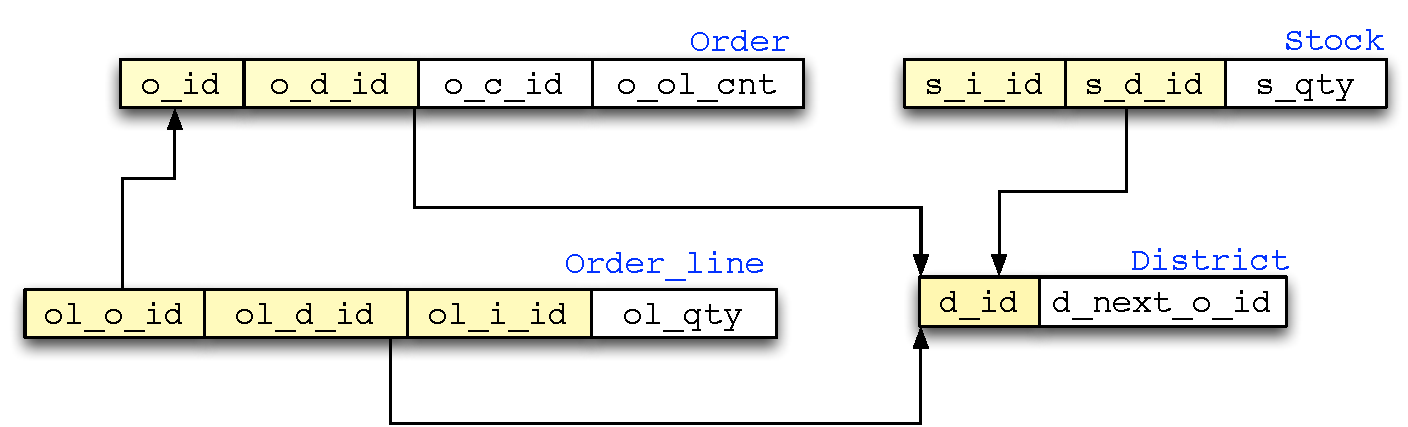
\includegraphics[scale=0.5]{Figures/schema}
\caption{Database schema of TPC-C's order management system.
  Columns against highlighted background are primary keys. Arrows denote
  foreign key relationships.}
\label{fig:schema}
\end{figure}

The \C{new\_order} transaction inserts a new \C{Order} record, whose
id is the sequence number of the next order under the given district
(\C{d\_id}). The sequence number is stored in the corresponding
\C{District} record, and updated each time a new order is added to the
system. Since each order may request multiple items (\C{item\_reqs}),
an \C{Order\_line} record is created for each requested item to relate
the order with the item. Each item has a corresponding record in the
\C{Stock} table, which keeps track of the quantity of the item left in
stock (\C{s\_qty}). The quantity is updated by the transaction to
reflect the processing of new order (if the stock quantity falls below
10, it is automatically replenished by 91).

TPC-C defines multiple invariants, called \emph{consistency
  conditions}, over the state of the application in the database. One
such consistency condition is the requirement that for a given order
\C{o}, the \emph{order-line-count} field (\C{o.o\_ol\_cnt}) should
reflect the number of order lines under the order; this is the number
of \C{Order\_line} records whose \C{ol\_o\_id} field is the same as
\C{o.o\_id}.  In a sequential execution, it is easy to see how this
condition is preserved.  A new \C{Order} record is added with its
\C{o\_id} distinct from existing order ids, and its \C{o\_ol\_cnt} is
set to be equal to the size of the \C{item\_reqs} set. The \C{foreach}
loop runs once for each \C{item\_req}, adding a new \C{Order\_line}
record for each requested item, with its \C{ol\_o\_id} field set to
\C{o\_id}. Thus, at the end of the loop, the number of \C{Order\_line}
records in the database, whose \C{ol\_o\_id} is equal to \C{o\_id} is
equal to the size of the \C{item\_req} set, which in turn is equal to
the \C{Order} record's \C{o\_ol\_cnt} field, thus preserving the
consistency condition.

Because the aforementioned reasoning is reasonably simple to perform
manually, verfiying the soundess of TPC-C's consistency conditions
would appear to be feasible.  Serializability aids the tractability of
verification by preventing any interference among concurrently
executing transactions while the \C{new\_order} transaction executes.
Under weak isolation\footnote{Weak isolation does not violate
  atomicity as long as the witnessed effects are those of committed
  transactions}, however, interferences of various kinds are
permitted.  Although the verification problem for weakly isolated
transactions would appear to be superficially similar to the
verification of (racy) concurrent programs (e.g., garbage
collectors~\cite{JLP+14,GHE15,HPQ+15}), weak isolation introduces new
challenges arising from the use of transactions, and new opportunities
arising from the fact that the store abstraction used by transactions
is a relational database, not low-level memory.

To illustrate some of these challenges, consider the behavior of the
\C{new\_order} transaction when executed with a \emph{Read Committed}
(RC) isolation level, the default isolation level in PostgreSQL, a
widely used open-source database system.  An RC transaction is
isolated from \emph{dirty writes}, i.e., writes of uncommitted
transactions, but is allowed to witness the writes of concurrent
transactions as soon as they are committed. Thus, with two concurrent
instances of the \C{new\_order} transaction (call them $T_1$ and
$T_2$), both concurrently placing new orders for different customers
under the same district (\C{d\_id}), PostgreSQL admits the two
executions shown in Fig.~\ref{fig:new_order_execs}.

\begin{figure}[!h]
\centering
\subcaptionbox {
  {\sc rc} Execution 1
  \label{fig:motiv-eg-1-b}
} [
  0.55\columnwidth
] {
  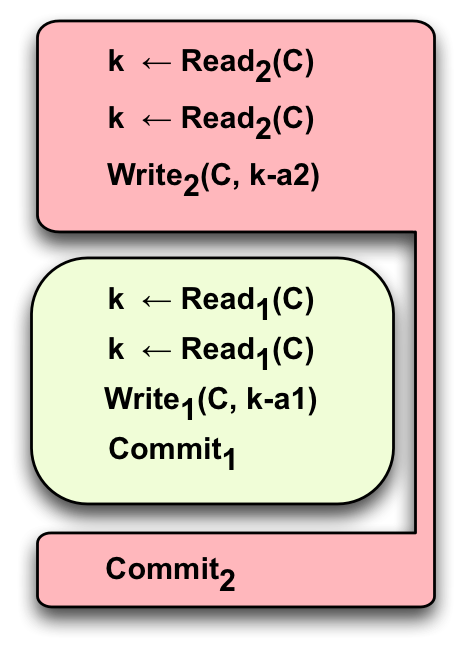
\includegraphics[scale=0.45]{Figures/motiv-eg-1-b}
}
%\hspace*{0.5in}
\subcaptionbox {
  {\sc rc} Execution 2
  \label{fig:motiv-eg-1-a}
}{
  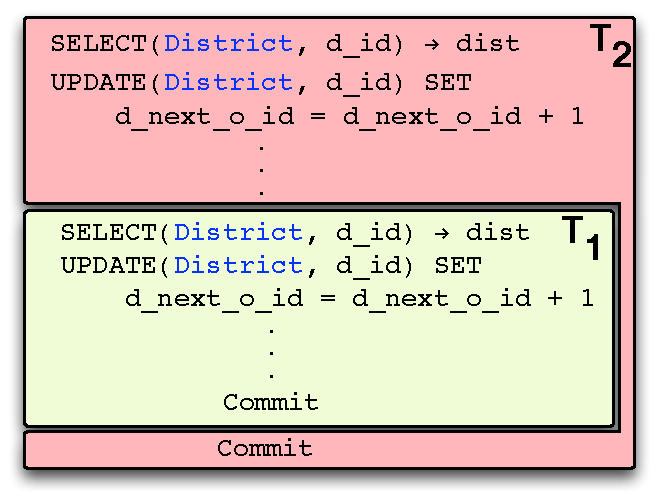
\includegraphics[scale=0.45]{Figures/motiv-eg-1-a}
}
  \caption{\small RC executions involving two instances ($T_1$ and
  $T_2$) of the \C{new\_order} transaction depicted in
  Fig.~\ref{fig:new_order_code}. 
  Each instance reads the \C{d\_id} \C{District} record twice, the second
  time to (atomically) update the \C{d\_next\_o\_id} field.}
\label{fig:new_order_execs}
\end{figure}

The figure depicts an execution as a series of transactional read, write, and commit
operations. In the execution on the left, the \C{new\_order} instance
$T_1$ (green) reads the \C{d\_next\_o\_id} field of the district
record for \C{d\_id}, but before it increments the field, another
\C{new\_order} instance ($T_2$) begins its execution and commits. Note
that $T_2$ reads the same \C{d\_next\_o\_id} value as $T_1$, and
inserts new \C{Order} and \C{Order\_line} records with their \C{o\_id}
and \C{ol\_o\_id} fields (resp.) equal to \C{d\_next\_o\_id}. $T_2$
also increments the \C{d\_next\_o\_id} field, which $T_1$ has already
acccessed. This is allowed because reads do not obtain a mutually
exclusive lock on most databases, including PostgreSQL. After $T_2$'s
commit, $T_1$ resumes execution and adds new \C{Order} and
\C{Order\_line} fields with the same order id as $T_1$. Thus, by the
end of the execution, \C{Order\_line} records inserted by $T_1$ and
$T_2$ all bear the same order id. There are also two \C{Order} records
with the same district id (\C{d\_id}) and order id, none of whose
\C{o\_ol\_cnt} reflects the actual number of \C{Order\_line} records
inserted with that order id.  This clearly violates TPC-C's consistency
condition.

Notably, this example does not exhibit any common concurrency bugs
that arise from incorrect use of weak isolation such as
\emph{write-write} conflicts, or \emph{lost updates}.  While $T_1$ and
$T_2$ both increment the \C{d\_next\_o\_id} field of the district
record, they do so atomically (Line 4 of
Fig.~\ref{fig:new_order_code}), allowing both updates to be present in
the final state. Likewise, other well-known anomalies that
characterize RC isolation~\cite{berenson} such as \emph{fuzzy reads},
\emph{phantom reads}, \emph{read skew}, and \emph{write skew}, are
also not exhibited by the example.  Thus, program analyses that aim to
determine appropriate isolation by checking for possible
manifestations of these anomalies would fail to identify grounds for
promoting the isolation level of \C{new\_order} to something stronger.
Yet, if we take the semantics of the application into account, it is
quite clear that RC is not an appropriate isolation level for
\C{new\_order}.

While reasoning in terms of anomalies is cumbersome, and as the above
example shows often inadequate, reasoning about weak isolation in
terms of low-level traces~\cite{adyaphd,gotsmanconcur15} complicates
high-level reasoning.  A possible alternative would interleave weak
isolation implementation details within the program, yielding a
(more-or-less) conventional concurrent program that can be then
subject to classical concurrent verification methods.  Considering the
size and complexity of real-world transaction systems, this strategy
is unlikely to scale.

In this paper, we adopt a different approach that \emph{lifts}
isolation semantics (\emph{not} their implementations) to the
application layer, providing a principled framework to simultaneously
reason about application invariants and isolation properties.  To
illustrate this idea informally, consider how we might verify that
\C{new\_order} is sound when executed under a \emph{Repeatable Read}
(RR) isolation level.  PostgreSQL executes an RR transaction by taking
a (conceptual) snapshot of the database state before the transaction
begins that is used by reads performing the transaction.  When the
transaction attempts to update a record, a check is made to determine
if the current version of the record in the database is the same as the
snapshot version. If it is, an exclusive lock is obtained on the
record, and the update is performed. If the record is already locked,
the transaction blocks until the lock is released.  When the lock is
obtained, is held exclusively until the transaction commits or rolls
back. If the aforementioned version check fails (i.e., the database
has a later version than the snapshot), the transaction is rolled back
and re-executed.

\begin{figure}[t]
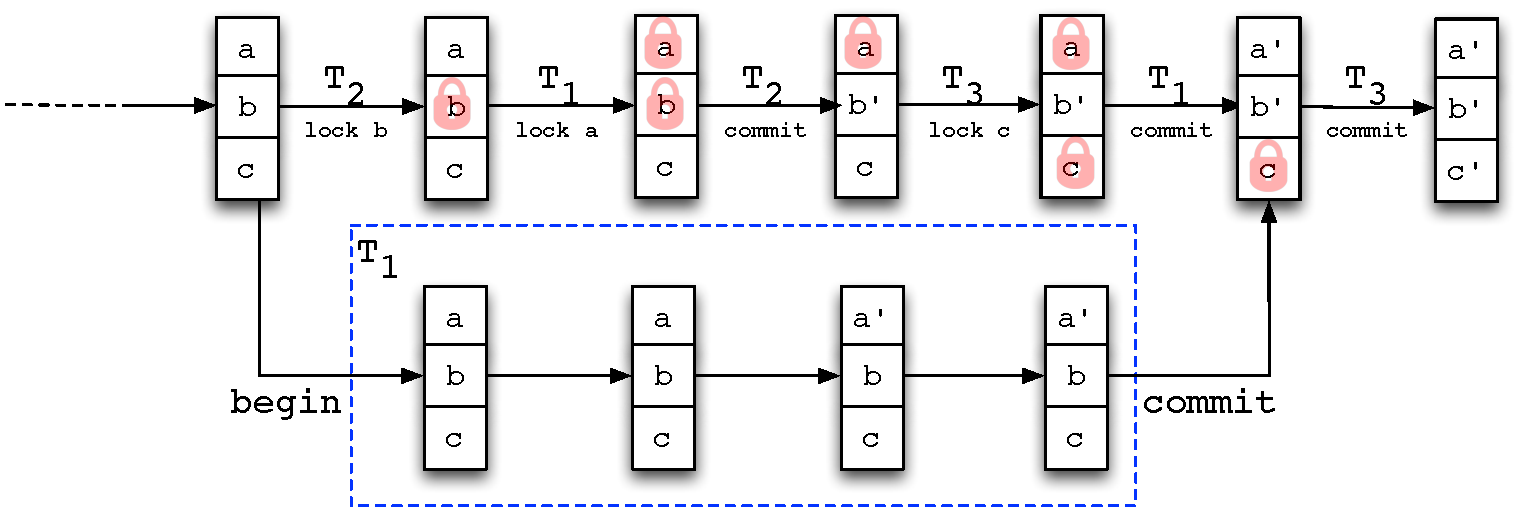
\includegraphics[scale=0.5]{Figures/RR-postgres}
\caption{Database state transitions corresponding to an execution of
  an RR transaction $T_1$ on PostgresSQL. $T_2$ and $T_3$ are concurrent
  transactions. The database state has three data items, $a$, $b$ and $c$. }
\label{fig:rr-postgres}
\end{figure}
\begin{figure}[t]
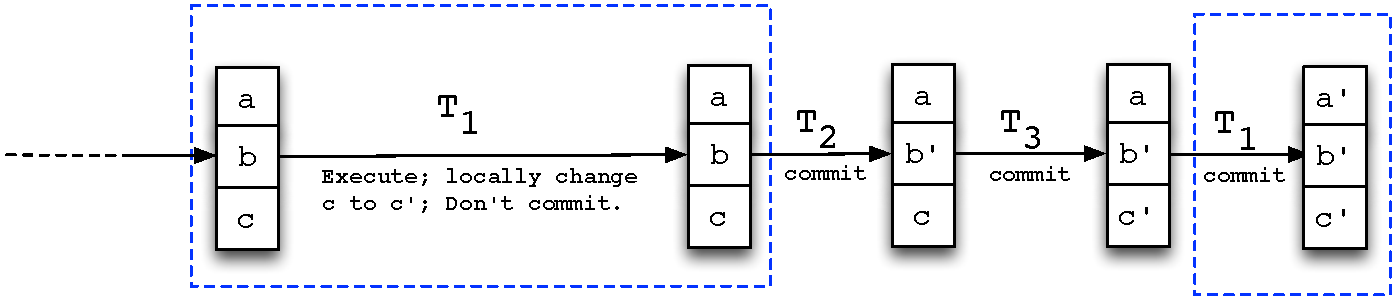
\includegraphics[scale=0.5]{Figures/RR-abstract}
  \caption{An abstract execution that includes the concrete execution
  shown in Fig.~\ref{fig:rr-postgres}. It has no locks or snapshots,
  admits fewer interleavings, yet results in the same post-state.  }
\label{fig:rr-abstract}
\end{figure}

Although this implementation, comprising many thousands of lines of
code, is highly involved, its semantic behavior in terms of how it
effects transitions on the database state is fairly simple.  Since a
transaction's reads are always served from a snapshot, no state
changes are witnessed while the execution is in progress. Thus,
insofar as an RR transaction is concerned, the database state does not
change during the execution.  Uncommitted writes are recorded in a
transaction-local state.  When the transaction commits, the local
state is atomically written to the global state to yield a global
state that reflects the transaction's updates.  However, unlike a
strongly isolated serializable transaction, the commit operation is
performed against the current state of the database, not the
snapshot. Thus, after the transaction finishes execution, but before
it commits, the transaction is able to witness the effects of all
concurrent transactions that committed before it.  The PostgreSQL RR
implementation effectively constrains this transition.

We can axiomatize this operational description by observing that (a)
due to the version check, the current transaction cannot update a data
item that was already updated by a concurrent transaction, and (b) due
to the use of exclusive write locks, a data item updated by the
current transaction cannot be overwritten by a concurrent transaction.
If $\Delta$ is the state of the database when an RR transaction
finishes, and $\Delta_c$ is the state visible to the transaction at
the point of commit, we know the transition from $\Delta$ to
$\Delta_c$ (written $\Delta \longrightarrow \Delta_c$) cannot exhibit
effects from any concurrent transactions that write to the same data
items as the current RR transaction.  Similarly, if $\delta$ denotes
a local log that relates transaction variables being written with their updated values,
then $\forall x\in\mathit{dom}(\delta)$, $\Delta_c(x) =
\Delta(x)$. To summarize, the operational semantics of PostgresSQL's RR
implementation can be captured as an axiomatization over transitions of
the database state ($\Delta \longrightarrow \Delta'$) during the
lifetime an RR transaction ($T$):
\begin{itemize}
  \item While $T$ executes, $\Delta' = \Delta$.
  \item After $T$ finishes execution, but before it commits its local
    state $\delta$, $\forall(x\in\delta).~\Delta'(x) = \Delta(x)$.
\end{itemize}

This simple characterization of RR isolation allows us to verify the
consistency condtions associated with the \C{new\_order}
transaction. First, since the database doesn't change ($\Delta' =
\Delta$) (where $\Delta'$ represents the state after the transaction
commits), during the execution of the transaction's body, we can
reason about \C{new\_order} as if it executed in complete isolation
until its commit point, leading to a verification process similar to
what would been applied when reasoning about serializability.  When
\C{new\_order} finishes execution and becomes ready to commit, a
transition that transfers the transaction'slocal writes ($\delta$) to
the unchanged database state ($\Delta$).  However, we are required to
consider the interference from concurrent transitions at this point,
which might change the database state from $\Delta$ to $\Delta_c$. If
this interference includes the effects of a concurrent \C{new\_order}
transaction (with the same \C{d\_id}), then verification fails as
described previously (Fig.~\ref{fig:new_order_execs}). Fortunately,
sequential reasoning shows that this is impossible - RR prevents a
concurrent \C{new\_order} transaction that modifies the same
\C{District} record as the current transaction (concretely, since the
record is already present in the current transaction's local log, any
transition from $\Delta$ to $\Delta_c$ cannot change this record).
Applying such axiomatic reasoning on \C{new\_order} allows us to prove
that the TPC-C invariant holds when the transaction is executed under
PostgreSQL's RR isolation.  Our proof framework generalizes this style
of reasoning to various isolation levels on databases.

The second observation that informs our approach is one that pertains
to automation. Program verification, even when machine-aided, often
entails significant annotation burden in the form of intermediary
assertions and loop invariants required to prove a program correct.
This is certainly true for concurrent program logics, such as
Rely-Gurantee, which extend Hoare logic with additional artifacts and
where (stable) intermediary assertions and loop invariants remain a
major source of annotation burden.  However, a relational database is
a significantly simpler abstraction than shared memory. There are no
pointers, or linked data structures, or aliasing.  Although a database
essentially abstracts a mutable state, the state is mutated through a
well-defined fixed number of interfaces (SQL statements), each tagged
with a logical formula describing what records are accessed and
updated. 

This observation leads us away from thinking of database transactions
as concurrent imperative programs.  Instead, we see value in viewing
them as essentially functional computations that manage database state
monadically. We find it useful to reason about
statements that mutate the database state, not in terms of a pre- and
post-condition pair, but in terms of a state transformer that relates
the pre- and post-states of a statement. This state transformer
semantics can be defined algorithmically, just like predicate
transformer semantics (e.g., strongest post-condition).  Here, a state
transformer interprets a SQL statement in the set domain, taking
advantage of the fact that a a database is essentially a set of
tuples, and a SQL statement is a transformer over these sets.  The
benefit of this approach is that low-level loops can now be
substituted with higher-order combinators that automatically lift the
state transformer of its higher-order argument (i.e., the loop body)
to the state transformer of the combined expression (i.e., the loop).
Thus the semantics of a \C{foreach} loop, for instance, can be
captured as a state transformer, where the state is a set, and the
transformation defines a bind operation. We illustrate this intuition
on a simple example.

% \begin{figure}[!t]
% \centering
% %
% \begin{subfigure}[b]{0.46\textwidth}
% \begin{ocaml}
% Set s' = $\emptyset$;
% foreach x in s {
%   s'.add(f(x)); 
% }
% \end{ocaml}
% \caption{}
% \end{subfigure}
% %
% \begin{subfigure}[b]{0.5\textwidth}
% \begin{ocaml}
% let s' = ref [];
% foreach s (fun x -> s' := x::(!s'));
% \end{ocaml}
% \caption{Lorem ipsum, lorem ipsum,Lorem ipsum, lorem ipsum,Lorem ipsum}
% \end{subfigure}
% \caption{Caption place holder}
% %
% \caption{New versions are created from existing versions either
% through \C{push} or \C{merge}.}
% \label{fig:syntactic-ancestors}
% \end{figure}
% let s' = ref (Set.empty) in
% foreach xs @@ fun x -> 
%   begin
%     s' := Set.union !s' @@ 
%             Set.map_selected s (fun y -> y<x)
%                                (fun y -> y+x);
%     s' := Set.add !s' x;
%   end
\begin{figure}[!h]
\begin{ocaml}
foreach item_reqs @@ fun item_req -> do
  SQL.update Stock (fun s -> {s with s_qty = k1}) 
                   (fun s -> s.s_i_id = item_req.ol_i_id);
  SQL.insert Order_line {ol_o_id=k2; ol_d_id=k3; 
                         ol_i_id=item_req.ol_i_id; ol_qty=item_req.ol_qty}
\end{ocaml}
\caption{Foreach loop from Fig.~\ref{fig:new_order_code}}
\label{fig:foreach_code}
\end{figure}

Fig.~\ref{fig:foreach_code} shows a (simplified) snippet of code taken
from Fig.~\ref{fig:new_order_code}. Some irrelevant expressions have
been replaced with constants (\C{k1} to \C{k3}).  The body of the loop
executes a SQL update followed by an insert.  Recall that a transaction
reads from the global database ($\Delta$), and writes to a
transaction-local database ($\delta$) before committing these updates. An update
statement filters the tuples that match the search criteria from $\Delta$
and computes the updated tuples that are to be
added to the local database. Thus, its state transformer (call it
$T_U$) is the following function on sets\footnote{$\bind$ has higher precedence than $\cup$.}:
\begin{ocaml}
  fun ($\Delta$,$\delta$) -> $\delta$ $\cup$ $\Delta$$\bind$(fun s -> if table(s) = stock && s.s_i_id = item_req.ol_i_id 
                                 then {{s with s_qty = k1}} (* a singleton set *)
                                 else $\emptyset$)
\end{ocaml}
% \begin{smathpar}
% \begin{array}{c}
%   \lambda\Delta.\lambda\delta.\, \delta \;\cup\; 
%       \Delta \,\bind\, (\lambda s.\, 
%           \C{if}\;{\C{stock}(s) \conj 
%                    \C{s.s\_i\_id} = \C{item\_req.ol\_i\_id}}\\
%            \hspace*{0.9in}
%            \C{then}\;{\{\{s \;\C{with}\; \C{s\_qty} = \C{k1}\}\}}\;
%            \C{else}\;{\emptyset})
% \end{array}
% \end{smathpar}
% \begin{verbatim}
%   Rmem(σ'(s')) = Rmem(σ(s')) U 
%                  Rmem[\x. Rmem[\y. if y<x then {y+x} else {}](σ(s)) U {x}](xs)
% \end{verbatim}
Observe that
$T_U(\Delta,\delta)$ is of the form $\delta \,\cup\,
F_U(\Delta)$. The transformer ($T_I(\Delta,\delta)$)
for the subsequent \C{insert} statement can be similarly calculated to
be of the form $\delta \cup F_I(\Delta)$.
Their composition gives the state transformer of the loop body:
\begin{ocaml}
  fun ($\Delta$,$\delta$) -> $\delta$ $\cup$ $F_U(\Delta) \,\cup\, F_I(\Delta)$
\end{ocaml}
Let $F_{body}(\Delta) = F_U(\Delta) \,\cup\, F_I(\Delta)$.   The
transformer for the \C{foreach} loop can now be computed as following:
\begin{ocaml}
  fun ($\Delta$,$\delta$) -> $\delta$ $\cup$ item_reqs$\bind$(fun item_req -> $F_{body}(\Delta)$)
\end{ocaml}
Observe that the transformer captures the precise semantics of the
loop as a formula in the domain of sets extended with a bind
function. The advantage in doing so is that we can now make use of a
semantics-preserving translation from this domain to first-order
logic, allowing us to leverage SMT solvers for automatic proofs
without having to infer loop invariant, or provide intermediate
assertions.  Sec.~\ref{sec:automation} describes this translation. In
the exposition thus far, we assumed $\Delta$ remains invaraint, which
is clearly not the case when we admit concurrency.  Necessary
concurrency extensions of the state transformer semantics is also
covered in Sec.~\ref{sec:automation}.  The following two sections,
however, focus on laying theoretical foundations for reasoning about
weak isolation.


% We recommend abbrvnat bibliography style.

\bibliographystyle{plainnat}
\small
\bibliography{all}

\end{document}
